% ex: ts=4 sw=4 sts=4 et filetype=tex
\begin{frame}
    \frametitle{Contenido}
    \tableofcontents
\end{frame}

\section{Sistema de Control de Versiones}

\begin{frame}[c]{Sin Sistema de Control de Versiones}
    \begin{center}
        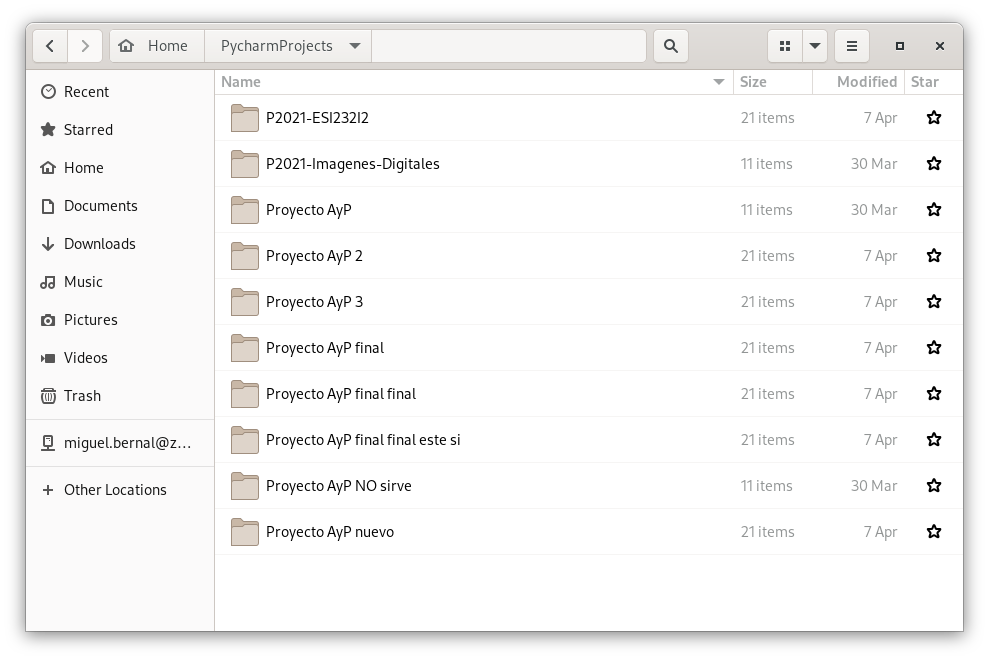
\includegraphics[scale=0.3]{img/proyectos-carpetas.png}
    \end{center}
\end{frame}

\begin{frame}[c]{Sistema de Control de Versiones}
    \begin{block}{Definición}
        Un control de versiones es un sistema que registra los cambios
        realizados en un archivo o conjunto de archivos a lo largo del
        tiempo, de modo que puedas recuperar versiones específicas más
        adelante.
    \end{block}

\end{frame}

\begin{frame}[c]{Sistema de Control de Versiones Locales}
    \begin{center}
        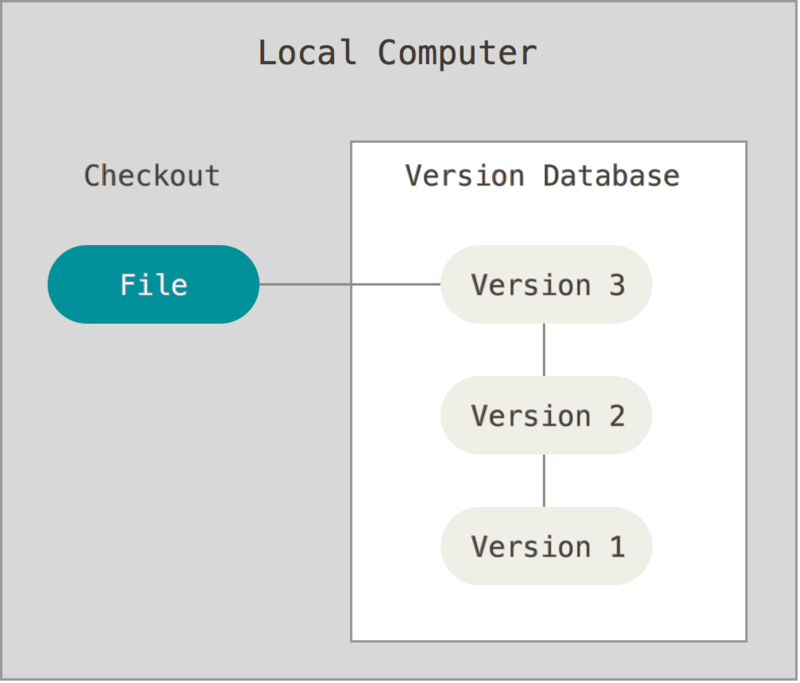
\includegraphics[scale=0.25]{img/scv-local.png}
    \end{center}
\end{frame}

\begin{frame}[c]{Sistema de Control de Versiones Centralizados}
    \begin{center}
        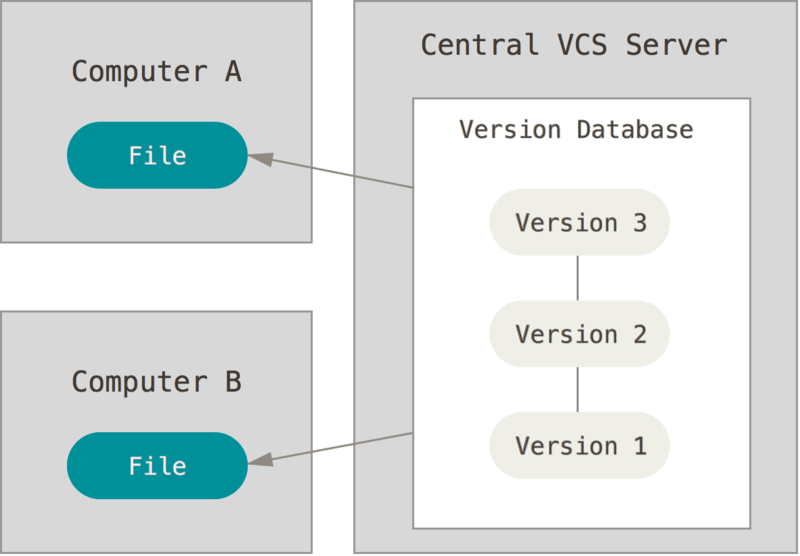
\includegraphics[scale=0.3]{img/scv-centralized.png}
    \end{center}
\end{frame}

\begin{frame}[c]{Sistema de Control de Versiones Distribuido}
    \begin{center}
        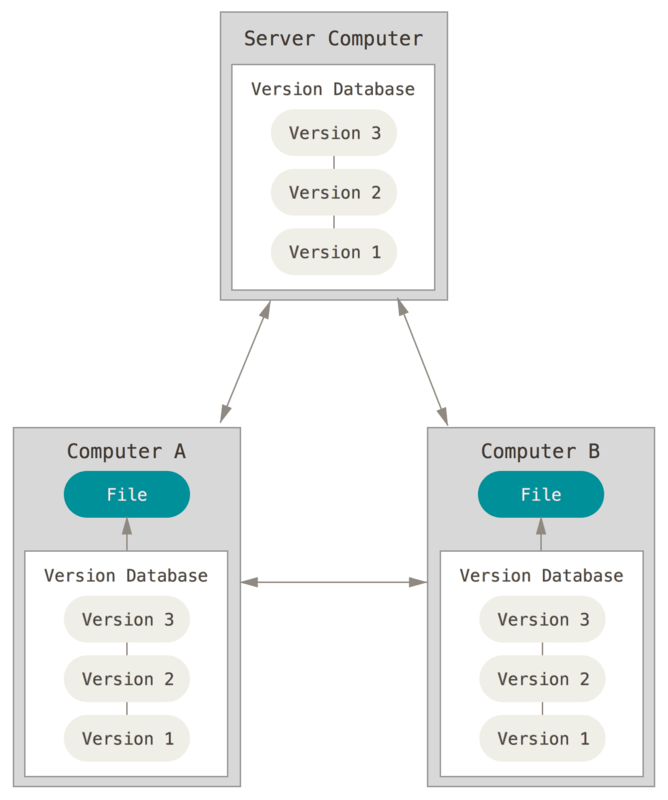
\includegraphics[scale=0.25]{img/scv-distributed.png}
    \end{center}
\end{frame}

\subsection{Git}

\begin{frame}[c]{Que es Git}
    \begin{columns}
        \column{0.5\textwidth}
        Git es un sistema de control de versiones distribuido, libre y de
        código abierto, diseñado para manejar todo, desde proyectos pequeños
        hasta muy grandes, con velocidad y eficiencia. 
        \column{0.5\textwidth}
        \begin{center}
            
\includegraphics[scale=0.5]{img/git-logo.png}
        \end{center}
    \end{columns}
\end{frame}

\begin{frame}[c]{Objetivos de Git}
    \begin{itemize}
        \item Velocidad
        \item Diseño sencillo
        \item Gran soporte para desarrollo no lineal (miles de ramas paralelas)
        \item Completamente distribuido
        \item Capaz de manejar grandes proyectos (como el kernel de Linux)
            eficientemente (velocidad y tamaño de los datos)
    \end{itemize}
\end{frame}

\section{Pycharm}

\begin{frame}[c]{Que es Pycharm}
    \begin{columns}
        \column{0.5\textwidth}
        PyCharm es un entorno de desarrollo integrado (IDE) utilizado en
        programación de computadoras, específicamente para el lenguaje Python.
        Está desarrollado por la empresa checa JetBrains (antes conocida como
        IntelliJ).
        \column{0.5\textwidth}
        \begin{center}
            
\includegraphics[scale=0.1]{img/pycharm-logo.png}
        \end{center}
    \end{columns}
\end{frame}

\begin{frame}[c]{Pantalla de inicio}
    \begin{center}
        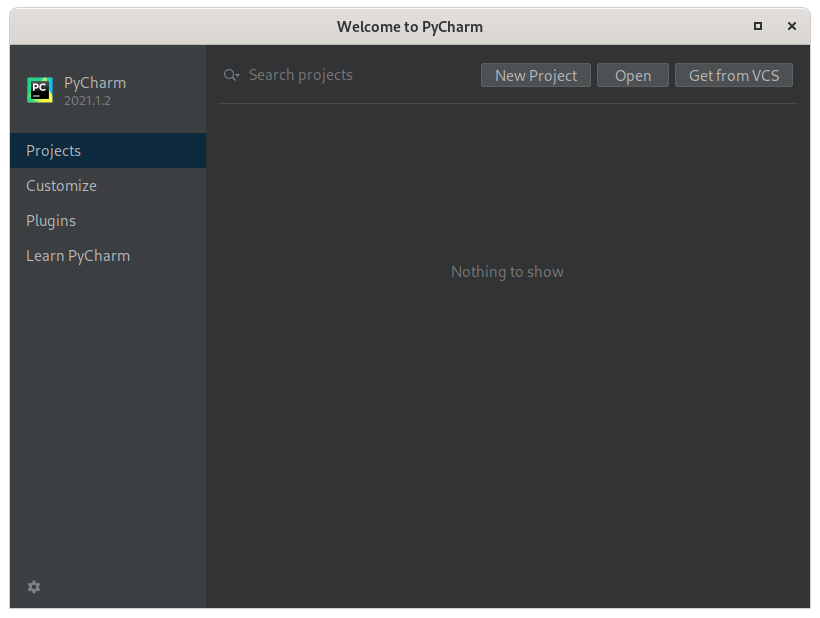
\includegraphics[scale=0.3]{img/pantalla-de-inicio.png}
    \end{center}
\end{frame}

\begin{frame}[c]{Obtenerlo por el Sistema de Control de Versiones}
    \begin{center}
        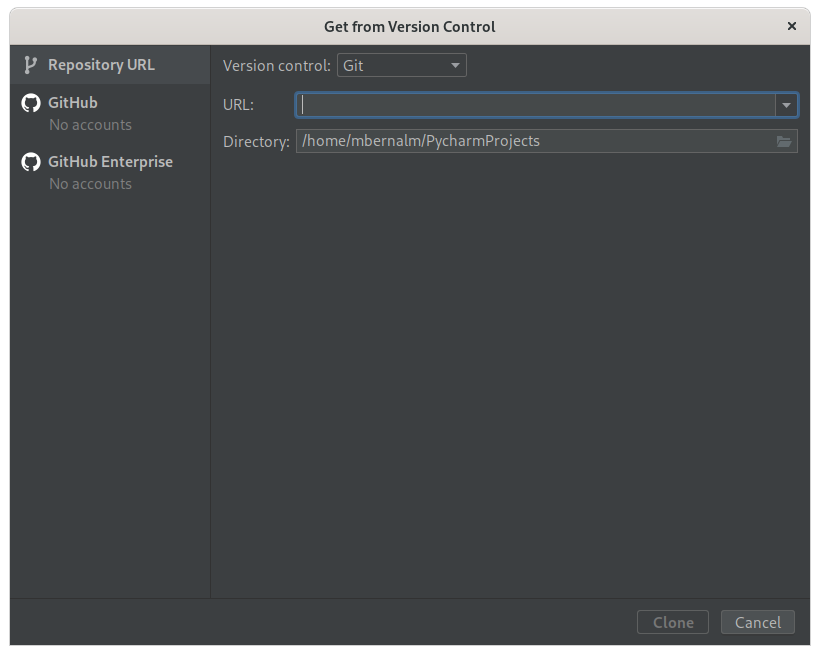
\includegraphics[scale=0.3]{img/get-from-vcs.png}
    \end{center}
\end{frame}

\begin{frame}[c]{Repositorio de Practica}
    \begin{center}
        \href{https://github.com/miguelinux/V2021-ESI232_T}{
            https://github.com/miguelinux/V2021-ESI232\_T}
    \end{center}
\end{frame}

\begin{frame}[c]{Clonar el repositorio}
    \begin{center}
        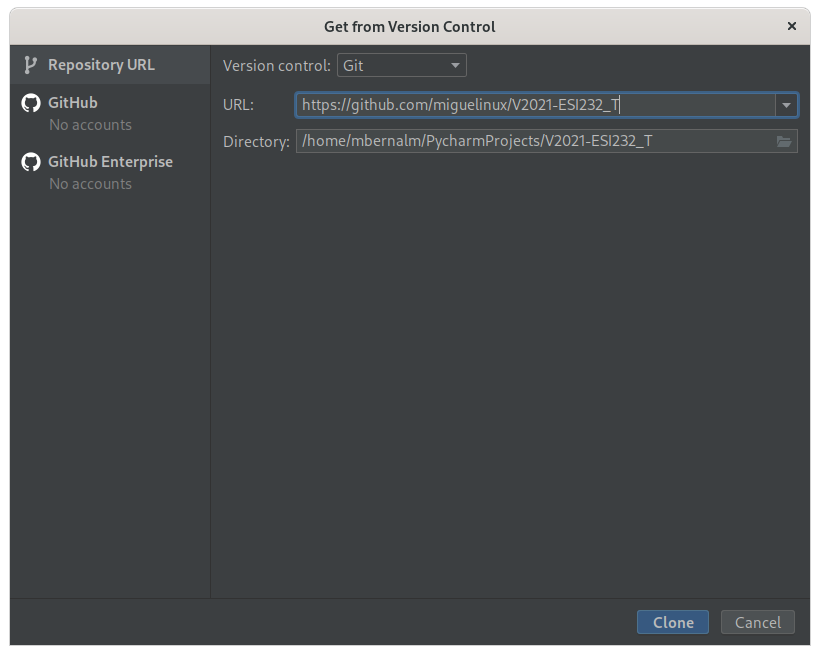
\includegraphics[scale=0.3]{img/url-to-clone.png}
    \end{center}
\end{frame}

\begin{frame}[c]{Ventana principal de proyecto}
    \begin{center}
        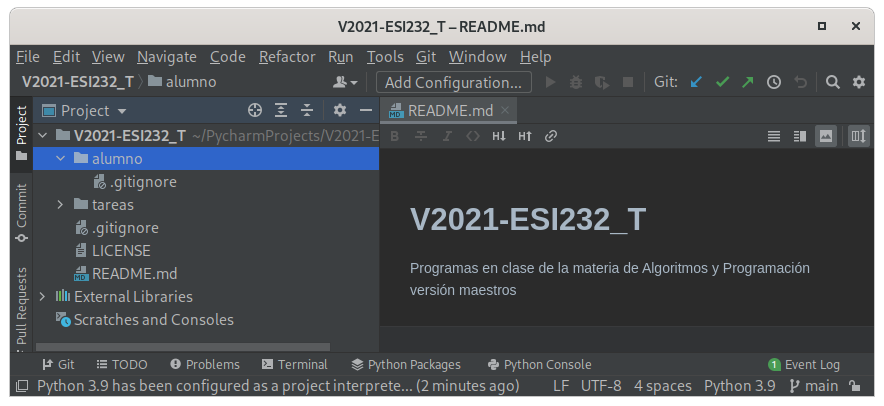
\includegraphics[scale=0.5]{img/clonado.png}
    \end{center}
\end{frame}


\section{GitHub}

\begin{frame}[c]{https://github.com}
    \begin{center}
        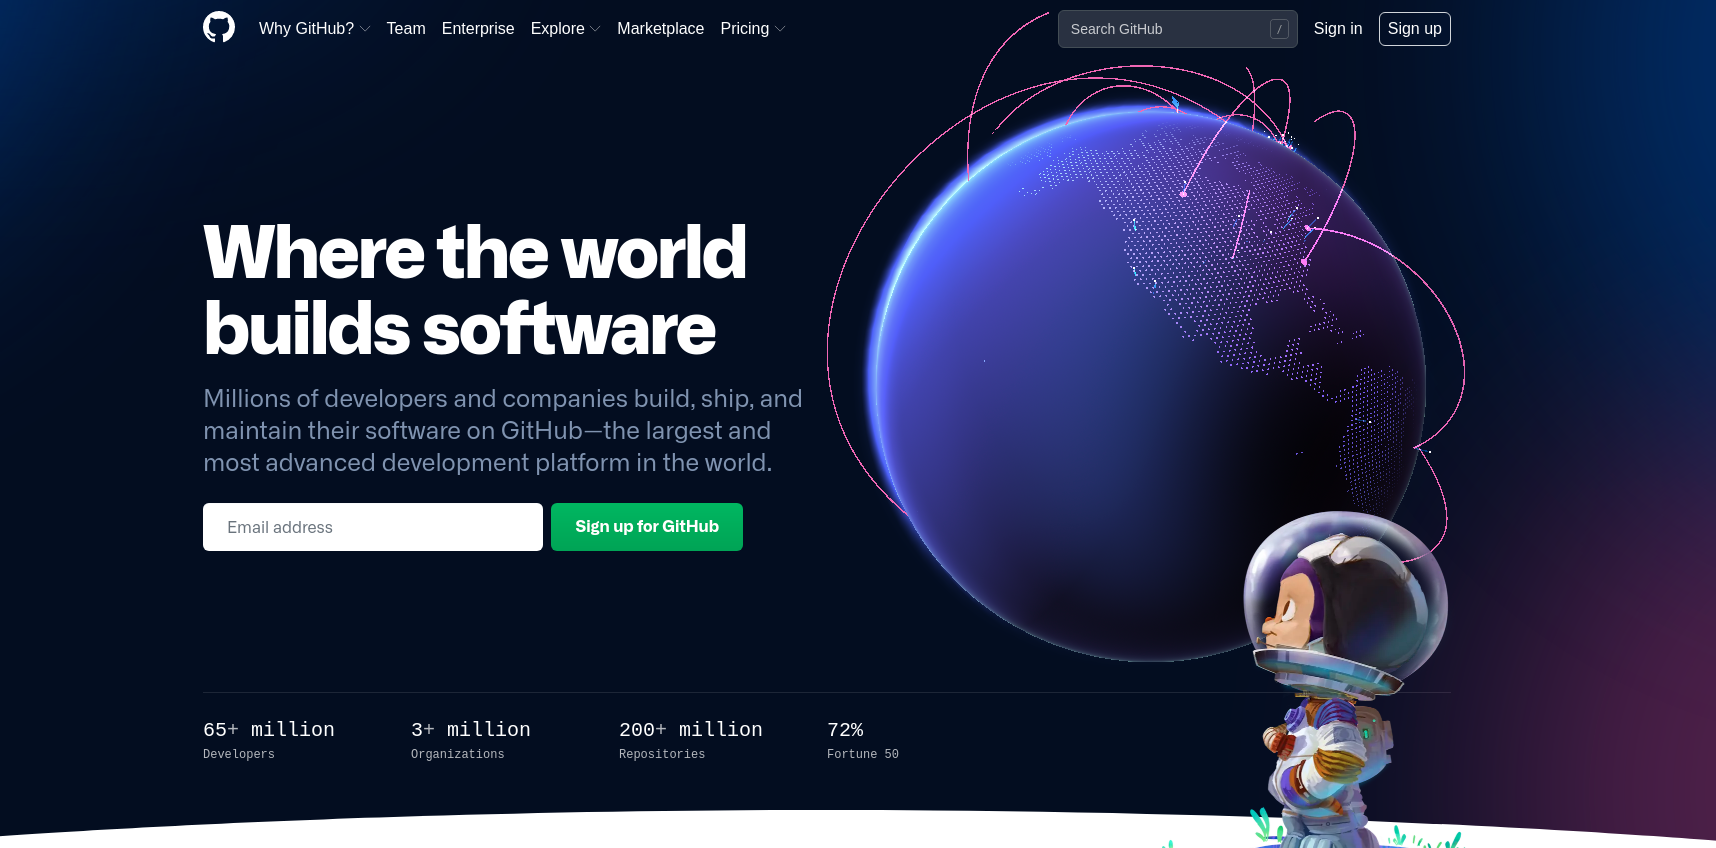
\includegraphics[scale=0.24]{img/github.png}
    \end{center}
\end{frame}

\begin{frame}[c]{Página de perfil}
    \begin{center}
        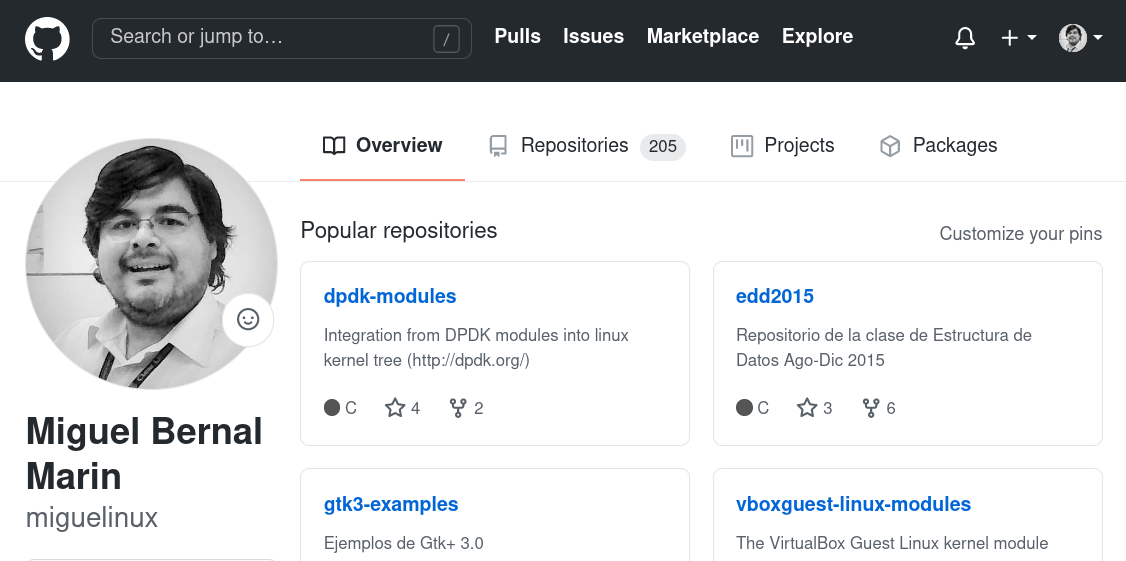
\includegraphics[scale=0.3]{img/github-profile.png}
    \end{center}
\end{frame}

\begin{frame}[c]{Menú más}
    \begin{center}
        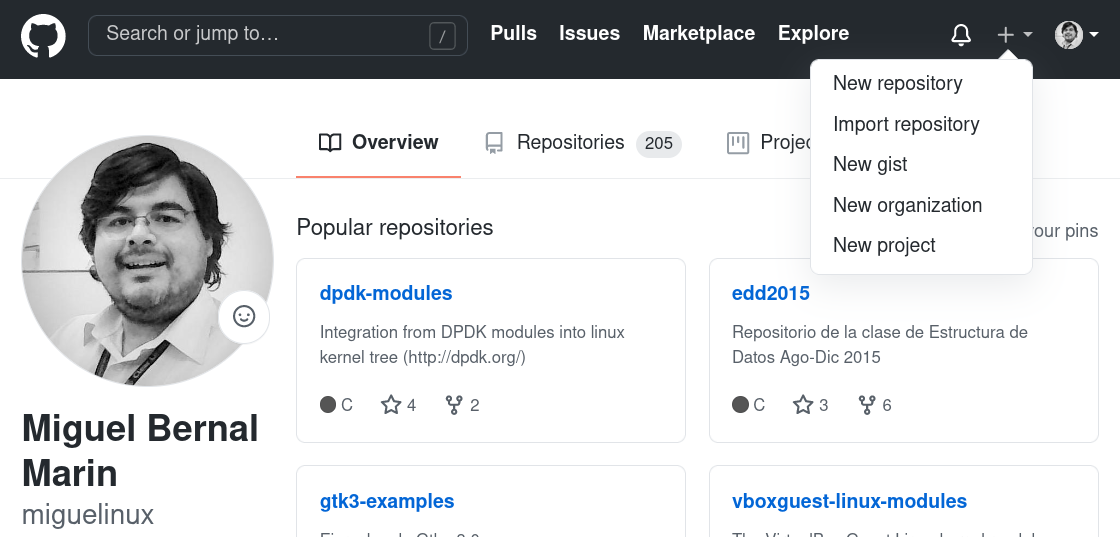
\includegraphics[scale=0.3]{img/github-plus-menu.png}
    \end{center}
\end{frame}

\begin{frame}[c]{Crear nuevo repositorio}
    \begin{center}
        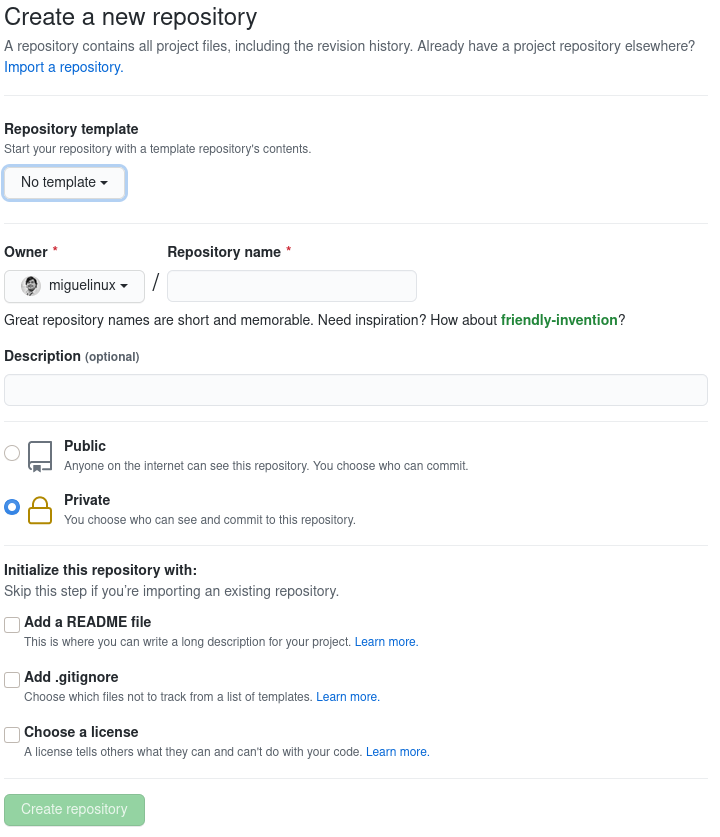
\includegraphics[scale=0.24]{img/github-new-repo.png}
    \end{center}
\end{frame}

\begin{frame}[c]{Página del repositorio}
    \begin{center}
        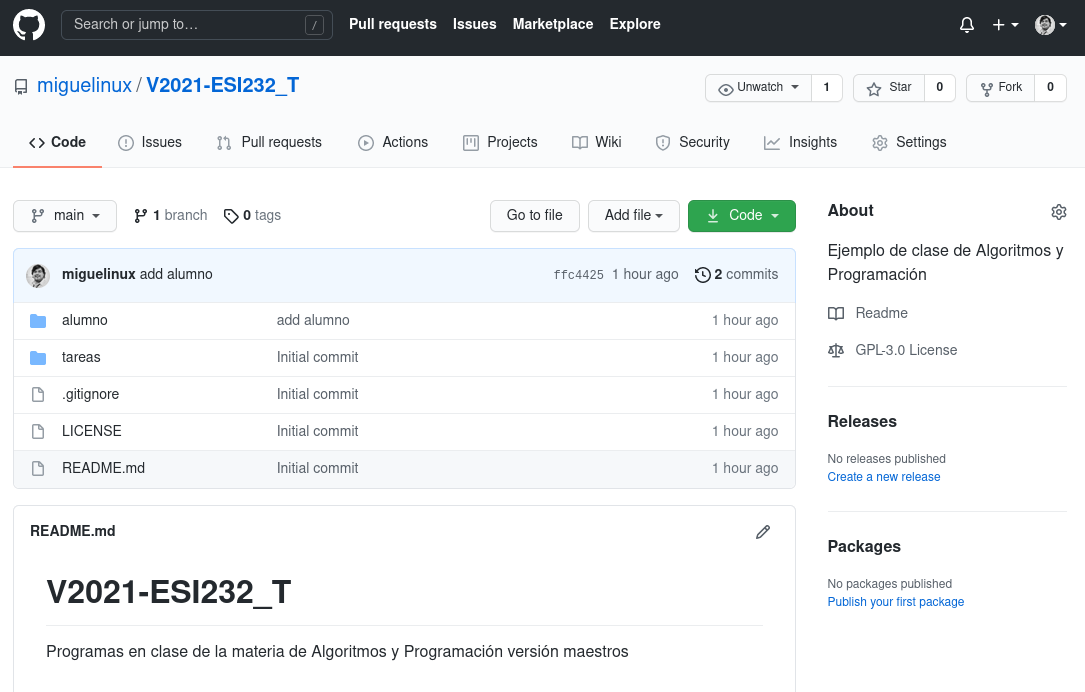
\includegraphics[scale=0.3]{img/github-repo.png}
    \end{center}
\end{frame}

\begin{frame}[c]{Configuración del repositorio}
    \begin{center}
        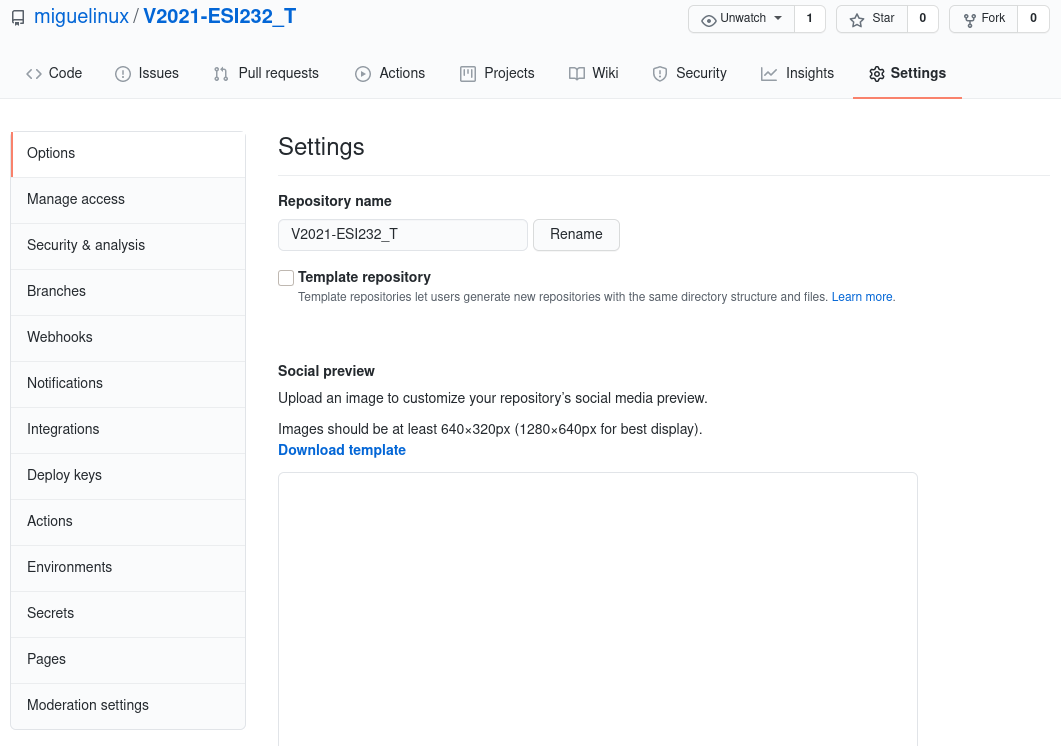
\includegraphics[scale=0.3]{img/github-repo-settings.png}
    \end{center}
\end{frame}

\begin{frame}[c]{Confirmación de password}
    \begin{center}
        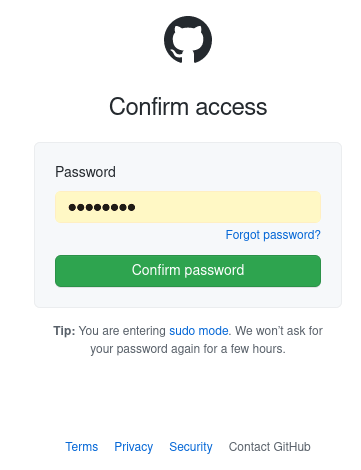
\includegraphics[scale=0.24]{img/github-ask-pwd.png}
    \end{center}
\end{frame}

\begin{frame}[c]{Administrador de accesos}
    \begin{center}
        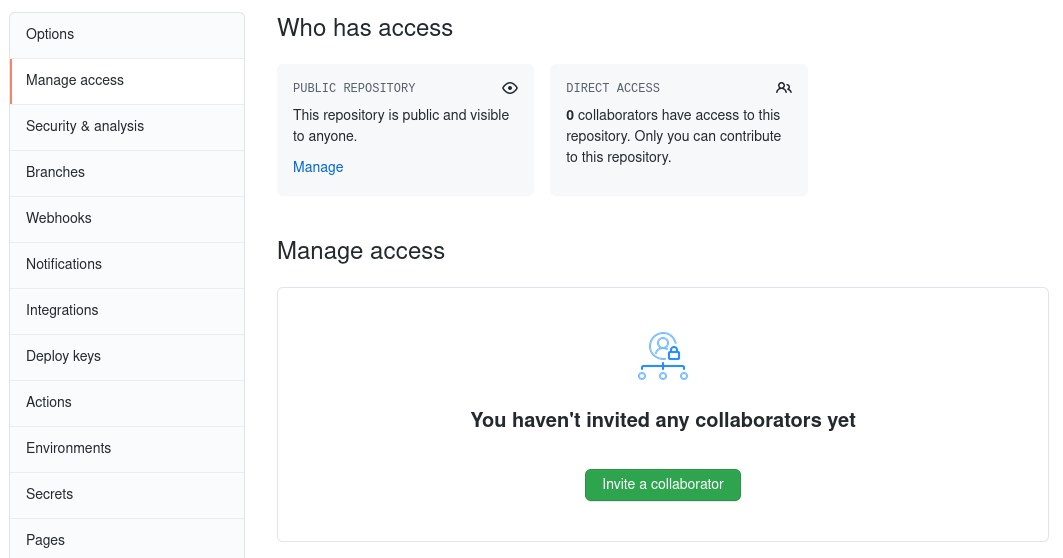
\includegraphics[scale=0.3]{img/github-manage-access.png}
    \end{center}
\end{frame}
